\input{../header}
\usepackage{pgfplots}
\rhead{Your name: \rule{8cm}{0.15mm}}

\begin{document}
%


%\onehalfspacing
\allowdisplaybreaks
%##################################################################
\section{Chapter 1 checkpoint!}

Hello and welcome to your first checkpoint! Here come five questions, one about each of the learning targets from Chapter 1. This is your scorecard:

\begin{center}
    \begin{tabular}{|m{3.75cm}|*{5}{m{2cm}|}} \hline
        Learning target: & DF1 & DF2 & DFa & DFb & AD2 \\\hline
        Your confidence level before starting (0-5): & &&&&\\\hline
        Your confidence level after the quiz (0-5): & &&&&\\\hline
        The mark you earned on this attempt: 
        & Success! \newline Try again!
        & Success! \newline Try again!
        & Success! \newline Try again!
        & Success! \newline Try again!
        & Success! \newline Try again! \\\hline

    \end{tabular}
\end{center}

Before anything else, please do the following:
\begin{itemize}
    \item Rank your confidence from 0-5 on each of the learning targets. 5 means ``I could teach a whole class about this;'' 0 means ``I am genuinely not sure I have heard these words before.''
    \item Write your name on this page and on each of the other pages of the quiz.
\end{itemize}

Then do the quiz! Some reminders:
\begin{itemize}
    \item Open notes, closed computer.
    \item If you need more room to write, use the back of the same learning target page, or ask me for some scratch paper.
    \item Read the questions carefully and make sure you're answering each part.
    \item Show all your work and explain all your thinking!
\end{itemize}

When you are done:
\begin{itemize}
    \item Rank your confidence from 0-5 on each of the learning targets. 5 means ``I absolutely nailed that question for sure;'' 0 means ``oof, I definitely didn't get that one.''
    \item Make double sure your name is on every page, including any scratch paper.
    \item Hand in your work, separated by learning target.
\end{itemize}

Have fun and do your best! I believe in u $\heartsuit$


%%%%%%%%%%%%%%%%%%%%%%%%%%%%%%%%%%%%%%%%%%%%%%%%%%%%%%%%%
\pagebreak
%%%%%%%%%%%%%%%%%%%%%%%%%%%%%%%%%%%%%%%%%%%%%%%%%%%%%%%%%
\section{Learning target DF1, version 1}


\everymath{\displaystyle}

Suppose that you know the following values of some function $g(x)$:

\[
\begin{array}{c||r|r|r}
      x  &  1.7 &  2   &  2.3 \\\hline
    g(x) & -2.2 & -2   & -1.5
\end{array}
\]
\begin{enumerate}[leftmargin=0pt]

\item Plot these points and sketch a plausible graph of $g(x)$.

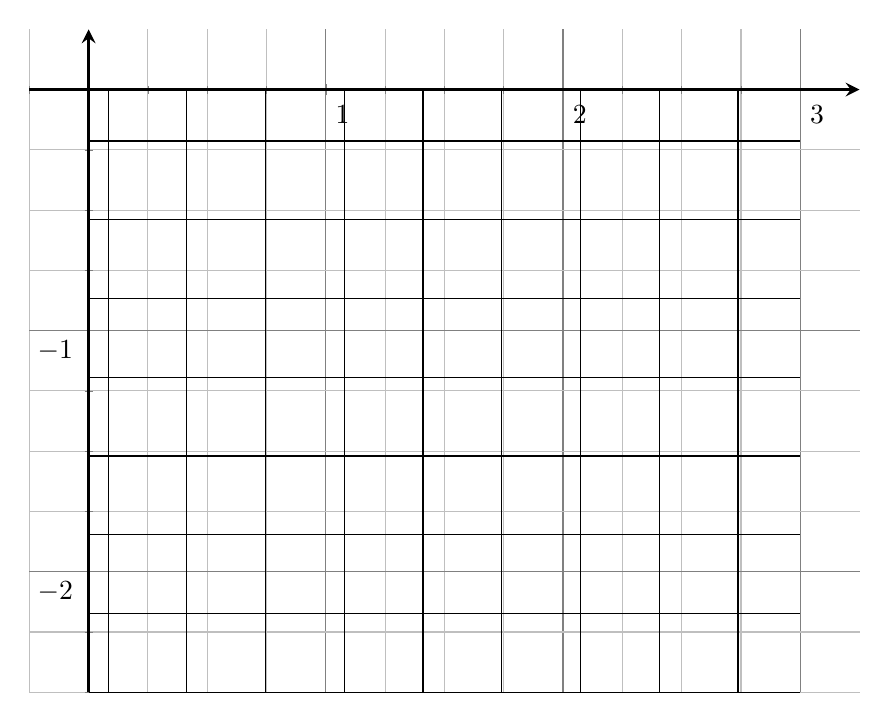
\begin{tikzpicture}
    \begin{axis}[
        width=\textwidth, height=10cm,
        xmin=-0.25, xmax=3.25, ymin=-2.5, ymax=0.25,
        xtick distance = 1, ytick distance = 1,
        minor tick num = 3,
        xticklabel style={anchor=north west},
        yticklabel style={anchor=north east},
        major grid style={thin, black!50},
        grid=both, 
        axis lines=center, axis line style = very thick]
        \draw (0,0) grid (3, -3);
    \end{axis}
\end{tikzpicture}

\item On your graph above, draw a plausible tangent line to the graph of $g(x)$ at $x=2$.

\item Use a central difference to estimate $g'(2)$. Draw the corresponding secant line on your graph above.

\vfill

\item Compute another estimate of $g'(2)$. Draw the corresponding secant line on your graph above.

\vfill

\item Which one of your approximations is the best? How do you know?

\vspace{1cm}

\end{enumerate}

%%%%%%%%%%%%%%%%%%%%%%%%%%%%%%%%%%%%%%%%%%%%%%%%%%%%%%%%%
\pagebreak
%%%%%%%%%%%%%%%%%%%%%%%%%%%%%%%%%%%%%%%%%%%%%%%%%%%%%%%%%

\section{Learning target DF2, version 1}

Suppose that $f(x) = 3x^2 - 5x + 4$.
\begin{enumerate}[leftmargin=0pt]
    \item Use the limit definition of the derivative to find $f'(x)$. \textbf{No shortcut rules!}
    
    \vfill
    \vfill

    \item Evaluate at $x=8$.

    \vfill
    \item (Bonus!) What happens to the 3? What about the $-5$? And the $4$?
\end{enumerate}

%%%%%%%%%%%%%%%%%%%%%%%%%%%%%%%%%%%%%%%%%%%%%%%%%%%%%%%%%
\pagebreak
%%%%%%%%%%%%%%%%%%%%%%%%%%%%%%%%%%%%%%%%%%%%%%%%%%%%%%%%%

\section{Learning target DFa, version 1}

A company manufactures rope, and the total cost of producing $r$ feet of rope is $C(r)$ dollars.
\begin{enumerate}[leftmargin=0pt]
    \item Suppose $C(2000) = 800$. Write a sentence explaining what this means, including units.
    \vfill
    \item What are the units of $C'(r)$?
    \vfill
    \item Suppose $C'(2000) = 0.35$. Write a sentence explaining what this means, including units.
    \vfill
    \item Do you think $C'(3000)$ is greater than, equal to, or less than $C'(2000)$? Explain why.
    \vfill
\end{enumerate}

%%%%%%%%%%%%%%%%%%%%%%%%%%%%%%%%%%%%%%%%%%%%%%%%%%%%%%%%%
\pagebreak
%%%%%%%%%%%%%%%%%%%%%%%%%%%%%%%%%%%%%%%%%%%%%%%%%%%%%%%%%

\section{Learning target DFb, version 1}

Here is the graph of some wacky function $q(x)$:

\begin{center}
    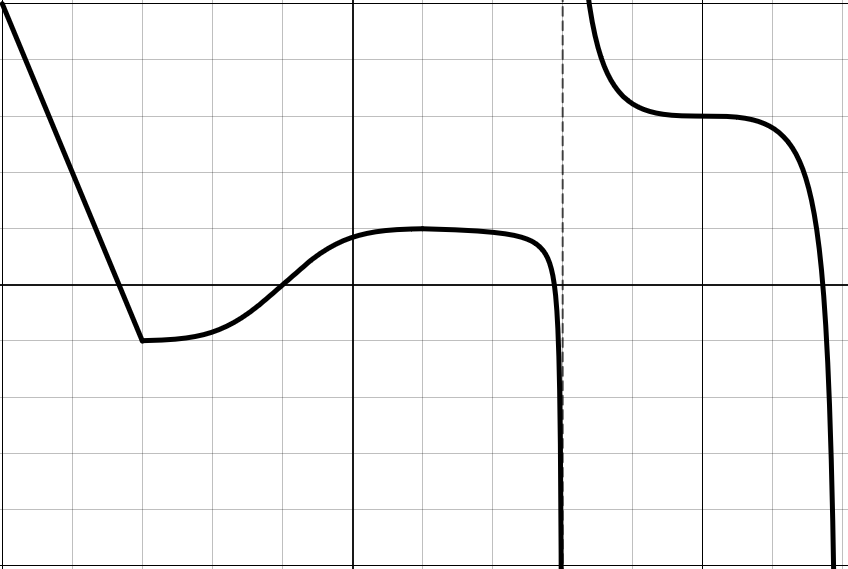
\includegraphics[width=0.9\textwidth]{../images/DFb-v1.png}    
\end{center}


Sketch the graph of $q'(x)$ on the blank axes below.

\begin{center}
    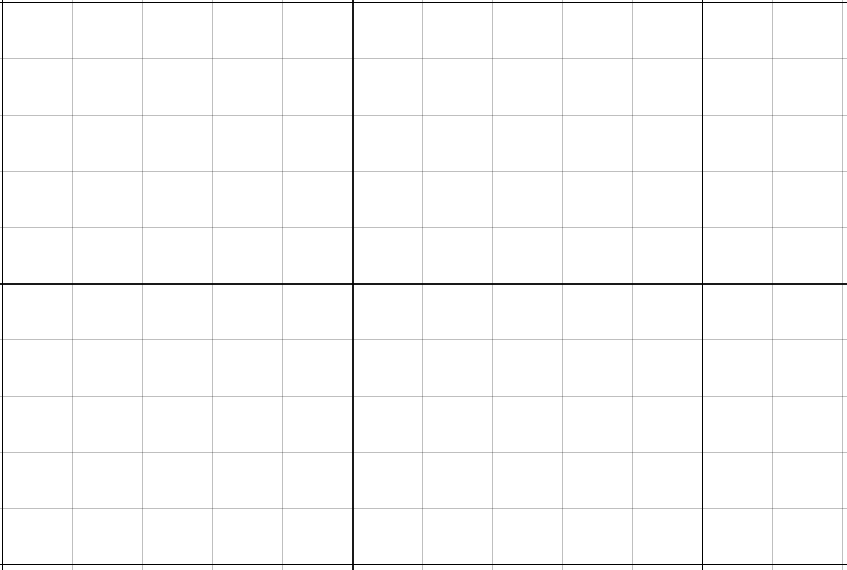
\includegraphics[width=0.9\textwidth]{../images/DFb-v1-blank.png}    
\end{center}


%%%%%%%%%%%%%%%%%%%%%%%%%%%%%%%%%%%%%%%%%%%%%%%%%%%%%%%%%
\pagebreak
%%%%%%%%%%%%%%%%%%%%%%%%%%%%%%%%%%%%%%%%%%%%%%%%%%%%%%%%%

\section{Learning target AD2, version 1}
Suppose that for some function \(p(x)\), you know the following information:
\begin{itemize}
    \item \(p(-2) = 5\),
    \item \(p'(-2) = 1.5\), 
    \item \(p''(x) < 0\) for \(x\)-values close to \(-2\). 
\end{itemize}

\begin{enumerate}[leftmargin=0pt]
    \item Explain and demonstrate how to find the linearization \(L(x)\) of \(p(x)\) at \(x =-2\). 
    \vfill
    \item Explain and demonstrate how to estimate the value of \(p(-2.03)\) using this linearization. 
    
    \vfill
    \item Is your estimate of \(p(-2.03)\) greater than or less than the actual value? How do you know?
    
    \vfill
    \item Sketch a possible graph of \(p(x)\) and its linearization \(L(x)\) nearby \(x =-2\) to illustrate your findings. Label important points in your sketch with their coordinates.
    
    \vfill
\end{enumerate}

\end{document}